\documentclass[9pt,twocolumn,twoside,lineno]{gsajnl}
% Use the documentclass option 'lineno' to view line numbers

%\articletype{inv} % article type
% {inv} Investigation 
% {gs} Genomic Selection
% {goi} Genetics of Immunity 
% {gos} Genetics of Sex 
% {mp} Multiparental Populations

\newcommand{\jri}[1]{\textcolor{blue}{[\begin{tiny}\textbf{JRI:} {#1}\end{tiny}]}}

\title{The Genetics of Phospholipid Metabolism In Maize Highland Adaptation}

\author[$\ast$,$\dagger$, 1]{Fausto Rodríguez-Zapata}
\author[$\dagger$, 1]{Karla Blöcher-Juárez}
\author[$\ddagger$]{Dan Gates}
\author[$\S$]{Li Wang}
\author[$\ast$]{Allison C Barnes}
\author[$\S$]{Garrett M Janzen}
\author[$\dagger$]{Rocío Aguilar-Rangel}
\author[$\dagger$]{Juan M Estévez-Palmas}
\author[$\dagger$]{Sergio Pérez-Limón}
\author[$\ast\ast$]{Oliver Fiehn}
\author[$\ddagger$]{Daniel Runcie}
\author[$\ddagger$]{Jeffrey Ross-Ibarra}
\author[$\S$]{Matthew Hufford}
\author[$\dagger$,$\dagger\dagger$]{Ruairidh JH Sawers}
\author[$\ast$,$\dagger$, 2]{Rubén Rellán-Álvarez}

\affil[$\ast$]{Department of Molecular and Structural Biochemistry, North Carolina State University, Raleigh, NC}
\affil[$\dagger$]{National Laboratory of Genomics for Biodiversity, Irapuato, México}
\affil[$\ddagger$]{Department of Ecology, Evolution, and Organismal Biology, Iowa State University, Ames, USA}
\affil[$\S$]{Department of Evolution and Ecology, Center for Population Biology and Genome Center, University of California, Davis, CA}
\affil[$\ast\ast$]{West Coast Metabolomics Center, University of California, Davis, CA, USA}
\affil[$\dagger\dagger$]{Department of Plant Science, The Pennsylvania State University, PA, USA}

\keywords{phospholipid metabolism; maize genetics; highland adaptation; convergent evolution}

\runningtitle{Phospholipid Pathway Selection in Highland Maize} % For use in the footer 

%% For the footnote.
%% Give the last name of the first author if only one author;
% \runningauthor{FirstAuthorLastname}
%% last names of both authors if there are two authors;
% \runningauthor{FirstAuthorLastname and SecondAuthorLastname}
%% last name of the first author followed by et al, if more than two authors.
\runningauthor{Rodríguez-Zapata, Blöcher-Juárez \textit{et al.}}

\begin{abstract}
After domestication from lowland teosinte in the warm, humid Mexican southwest maize colonized the highlands of Mexico and South America. In the highlands, maize was exposed to a whole range of environmental factors that differ from the site of domestication, including, among others, lower temperatures, soils with lower phosphorus availability and different biological pressures. In my talk, I will present data supporting the hypothesis that glycerolipid metabolism remodeling was important in the process of maize adaptation to highlands. I will show results from common garden experiments in Mexican lowland and highland common gardens where we grew maize mapping populations and using quantitative biochemical genetics tools we identified major QTLs that explain the conversion of phosphatidylcholines (PCs) to lyso-phosphatidylcholines (LPCs) leading to a high PC/LPC ratio that is particularly conserved in Mexican highland landraces. Using GBS data from 4000 maize landraces and whole genome sequences from another 30 landraces across the Americas we found that candidate genes underlying this QTL and others coding for PCs to/from LPCs conversions also show clear signs of selection to highlands. I will present ongoing work to identify the causative SNPs on candidate genes that lead to this biochemical phenotype, their natural variation and ultimately the physiological mechanisms that are affected by it and their role in maize highland adaptation. 
\end{abstract}

\begin{document}

\maketitle
\thispagestyle{firststyle}
%\marginmark
\firstpagefootnote
\equalcontrib{1}
%\equalcontrib{2}

\correspondingauthoraffiliation{3}{Department of Molecular and Structural Biochemistry, North Carolina State University, 27607, Raleigh, NC. Email: rrellan@ncsu.edu}
\vspace{-33pt}% Only used for adjusting extra space in the left column of the first page

\section{Introduction}

\lettrine[lines=2]{\color{gray}M}aize (\textit{Zea mays spp. mays}) was domesticated in the tropical basin of the Balsas River (Guerrero, Mexico) around 10,000 years ago from the wild relative teosinte parviglumis (\textit{Zea mays spp. parviglumis}) \citep{Matsuoka2002-bg,Piperno2009-fj}). 
After domestication, maize expanded throughout México, north into the US \citep{Da_Fonseca2015-zh} and south into Central America and South America (Wang et al., 2017) and has been adapted to a wide diversity of environments and today is grown in a wider geographical range than any other crop \citep{Hake2015-or}.  
Maize has also adapted to a wide variety of uses, from the myriad culinary applications of local communities growing maize landraces particularly in Mexico \citep{Bellon2018-cm} to the diverse range of products (from ethanol to high fructose syrup) that are produced with modern hybrids in modern agronomical operations. 
The genetic changes that lead to maize domestication \citep{Doebley1995-su,Doebley1997-oy, Wang2005-by, Clark2006-xh,Dorweiler1993-ik} and maize adaptation to a wider latitudinal range \citep{Liang2018-af, Guo2018-on, Coles2010-db, Huang2018-ga, Yang2013-lg, Salvi2007-ku, Wang2017-bc} provide a relatively good understanding of the genetic regions and mechanism that shaped maize domestication and latitudinal expansion. 
However, the mechanisms involved in maize landrace local adaptation that enabled maize to adapt to such a diverse range of environmental conditions are still largely unknown. 

In this paper, we posit  phospholipid pathways are under selection in highland balance had an important role in maize adaptation to highlands.  
Our hypothesis is based on what we know about how plants respond to a number of environmental conditions that are characteristic of highlands and that affect phospholipid metabolism and conferred an adaptive significance as maize colonized highland territory. 
Phospholipid concentration increases \citep{Degenkolbe2012-wf} together with a reduction of glycerolipids with highly saturated fatty acids \citep{Welti2002-uk} are two of the strategies plants use to respond to cold temperatures \cite{Lynch1987-ln}. 
These changes are supposed to help maintain the fluidity of plasma membranes at colder temperatures. On the other hand, plants adapted to low phosphorus conditions degrade phospholipids and increase the concentration of glycerolipids and sulpholipids (Lambers et al., 2012), particularly, in older leaves to free up phosphorus. 
The highlands of Mexico, and particularly the Trans-Mexican volcanic belt are characterized volcanic soils with low phosphorus availability (Krasilnikov, P., Gutiérrez-Castorena, M.d.C., Ahrens, R.J., Cruz-Gaistardo, C.O., Sedov, S., Solleiro-Rebolledo, E, 2013). 
In the regions where maize is grown in Mexico, there is a positive correlation between altitude and phosphorus retention (Zapata, 2018). 
As maize adapted to higher elevations with lower phosphorus availability and colder temperatures, phospholipid metabolism faced contrasting selective pressures. 

Cold temperatures also affect maize development. Farmers can predict flowering dates using Growth Degree Units (GDU) that takes into account the maximum and minimum temperatures on a given day. 
Maize needs between 800 and 1400 GDU to reach maturity. 
In Mexican highland conditions, growing degree days are usually around 5 GDU while in lowlands they are 15 GDU. 
It takes a maize plant around 3 times longer to reach maturity in highland than in lowland conditions. To deal with these lower GDUs, highland maize landraces are planted early in the season (February-March) and harvested around November. 
Highland adapted landraces have short flowering times probably as an adaptive strategy to deal with low GDU values in the highlands.  
In maize, glycerolipid content has a high flowering time predictive power (Riedelsheimer et al., 2013). 
The high predictive predictive power of flowering time by glycerolipids could be explained at the molecular level by the discovery that certain phosphatidylcholine species bind to flowering locus T and accelerate flowering time through a yet unknown mechanism (Nakamura et al., 2014). 
 
Several lines of evidence indicate that glycerolipid metabolism was under selection in independent events of maize highland adaptation. 
Takuno and collaborators used Fst statistics to identify loci that were under selection in both Mesoamerica and South America highland maize (Takuno et al., 2015). 
They found little evidence of convergence between the two sub continents but glycerolipid pathways were under the few pathways that showed convergence at the pathway level (Takuno et al., 2015). 

In this paper we set out to study the possible role glycerolipid and in particular phospholipid metabolism in the process of maize adaptation to highland conditions. 
Using a multi pronged approach that combined QTL analyses of phospholipid content biparental RIL mapping made of a cross of B73 and Palomero Toluqueño (a highland landrace), phospholipid analysis in a 120 landrace diversity panel, analysis of genome wide signals of selection to highland altitude using WGS of 30 landraces and GBS data of 2700 landraces we identified candidate loci  that were both under selection in highland maize and that show phospholipid quantitative variation  in biparental populations. 

In particular, our analysis identified a major QTL controlling phosphatidylcholine and lyso-phosphatidylcholine levels. A phospholipase type A1 (\textit{ZmPla1.2}) that shows strong signals of selection in highland maize and is located at the peak of the QTL. Further analysis using the genetic materials generated in this paper will allow us to test the adaptive significance of this metabolic trait to maize adaptation to highland conditions and will help to better understand if natural variation in the candidate loci could be used to improve modern maize varieties that face similar environmental conditions than highland maize like early season cold stress. 
\section{Results}
\label{sec:results}

\subsection{Glycerophospholipid pathways are under selection in  highland maize} 
We analyzed selection of glycerolipid related pathways in highland maize using several approaches. 
We first identified glycerolipid related pathways in Kegg and the Plant Metabolic Network \cite{Schlapfer2017-yl}. We identified 29 pathways with a total of 594 genes. 
We used this list to analyze if the enzymatic pathways involved in determining the glycerolipid makeup of maize are under selection in highland maize and also the extent of possible convergent selection across different maize highland regions. 
We were particularly interested in identifying possible patterns of convergent selection in maize populations that have adapted independently to highland conditions (Figure \ref{Fig1}A).  

We then used the Population Branch excess (PBE) statistic \cite{Pool2017-oa} and applied it to four highland populations (Southwest US, Mexican Highland, Guatemalan Highlands and Andes). 
Each group contains three to six accessions from that particular area and have been sequenced at an average 30X coverage \cite{Wang2017-bc}. 
In short, PBE quantifies changes in allele frequencies in focal populations relative to two independent “outgroup” populations. We used \textit{teosinte parviglumis} as one of the outgroup populations for all four highland groups. 
The other outgroup was Mexican lowlands in the case of SW US, Mexican highlands and Guatemalan highlands, and South American lowlands in the case of the Andes Populations. A SNP was classified as a potential target of selection if it was in the top 5\%. 
\begin{figure*}[ht]
\begin{center}
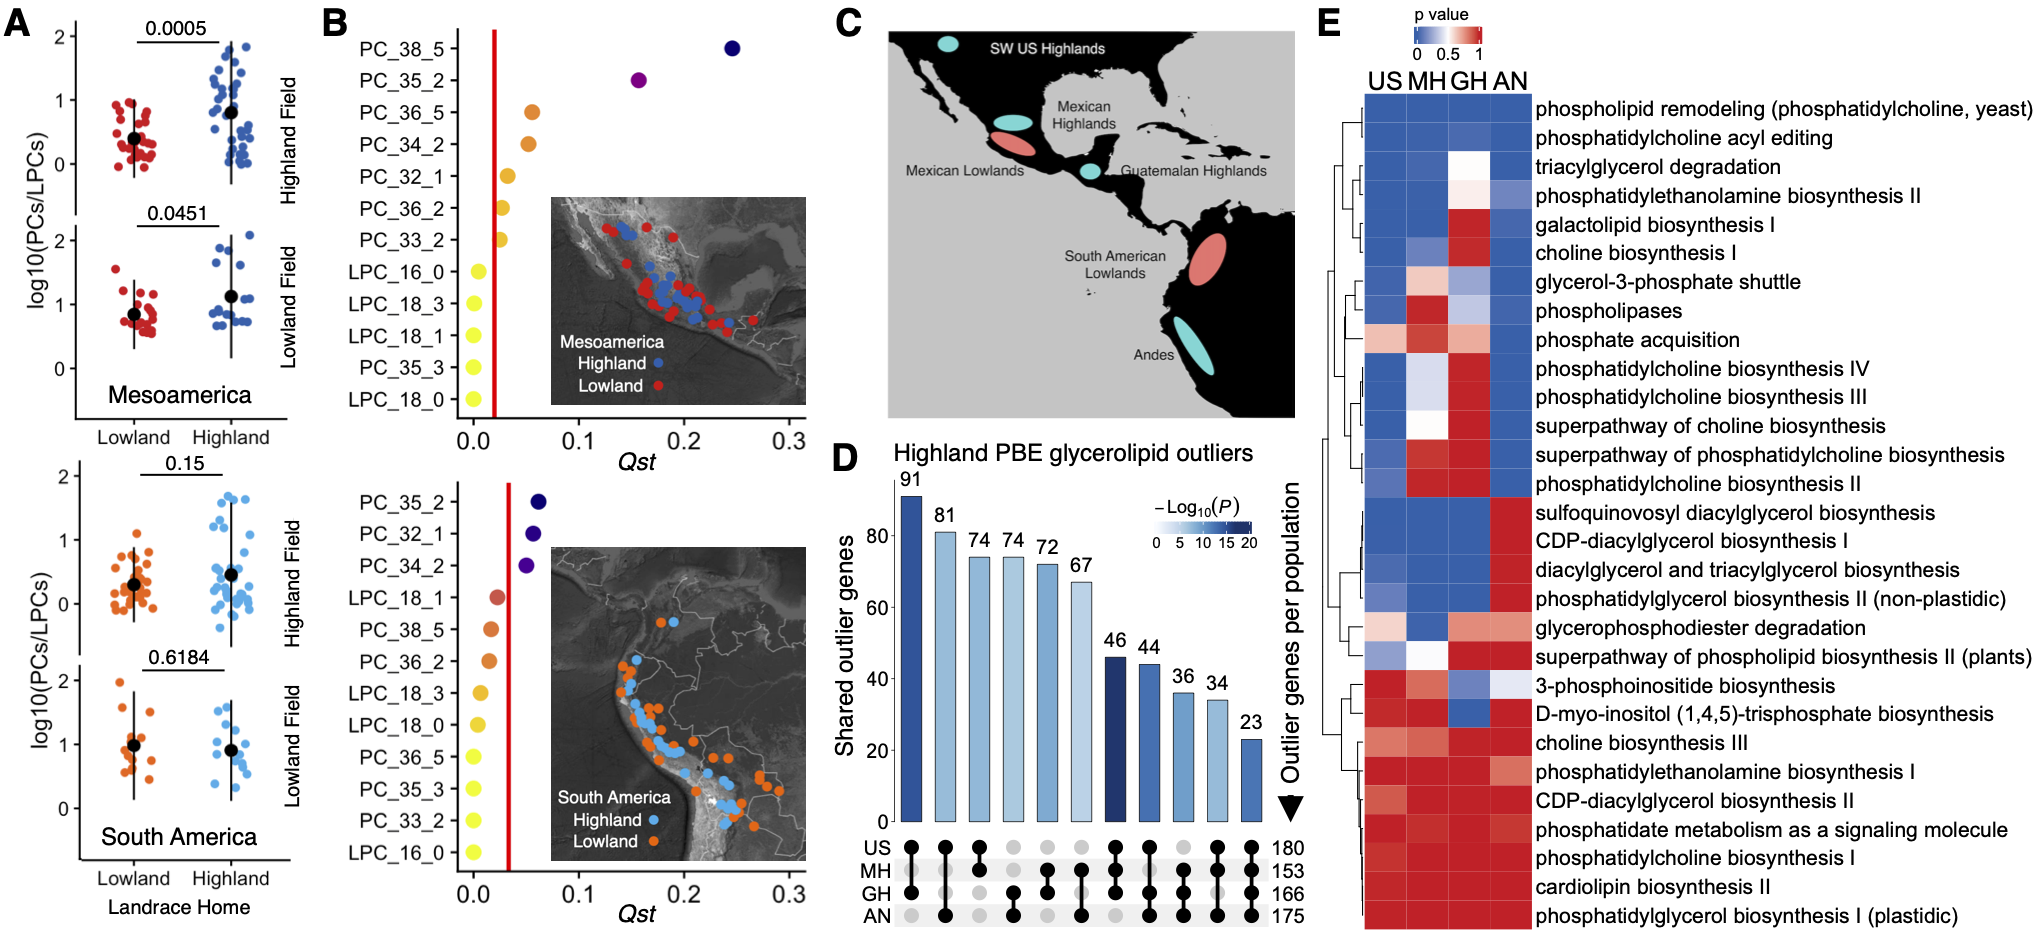
\includegraphics[width=0.8\paperwidth]{Figures/Fig_1.png}
\caption{Glycerolipid pathway selection 
A) Populations used in the Population Branch Excess (PBE)analysis. 
B) Average PBE values within genes and 10KB windows upstream and downstream of the gene of each pathway were compared against random genome wide sample of the same number of genes. The heatmap shows p-values of a (indicate what type of test) for each pathways. 
C) PBE values of SNPs in\textit{ZmLpcat1}and\textit{ ZmPla1.2}across SWUS, Mexican Highlands, Guatemalan Highlands an Andes populations (from top to bottom). Dark shade rectangles mark the coding sequence of each gene. Light shading rectanles on the borders of the coding sequence mark 10KB upstream and downstream windows. 
D) Map showing the geographical origin of the 120 accessions used in the common garden experiment to quantify glycerolipid compounds.
E) Correlation between  lyso-phosphatydilcholine (LPC) species and the ratio of  phosphatydilcholine (PCs) species and LPC species. 
F) Logaritmic values of the PC34:1/LPC18:1 ratio of highland and lowland landraces from Mesoamerica and Southamerica}
\label{Fig1}
\end{center}
\end{figure*} 
A genome wide PBE analysis of the same populations \cite{Wang2017-bc} found strong indications of convergent adaptation to highland environments across all four populations at the SNP, gene and pathway level.
Within the list of 594 we identified a significant excess of genes that were target of selection in more than two populations (p < 2.87e – 5, Figure \ref{SupFig1}A). This excess was particularly strong (p < 2.87e – 5, Figure \ref{SupFig1}A) in the SWUS, Mexican and Guatemalan Highland populations. 
These three populations also showed the highest number of genes that recurrently selected in all populations. 
There were 22 genes that were selection outliers in all four populations. 

We then performed an independent analysis for each of the 29 pathways and compared the average PBE value for SNPs 10kb windows around genes in that pathway with a genome wide random sampling distribution. Pathways involved in phosphatydilcholine (the most abundant phospholipid species) remodelling were significantly enriched in selection outlier genes across all 4 populations indicating an adaptive role of phospholipid remodelling in maize highland adaptation (Figure \ref{Fig1}B, Supplementary Fig1B).
Pathways involved in triacylglycerol degradation and galactolipid biosynthesis were recurrently selected in the SWUS, Mexican Highlands and the Andes while others involved in sulpholipid and diacylglycerol and phosphatidylglycerol biosynthesis were selected in the SWUS and mesoamerican populations (Figure \ref{Fig1}B).  

\textit{ZmLpcat1} (lyso-phosphatydilcholine acyl transferase 1) is an example of a gene selected in all four populations that is part of the phospholipid remodelling and phosphatydilcholine acyl editing pathways. 
It contains several outlier SNPs within the codins sequence of the gene that are shared across all four highland populations (Figure \ref{Fig1}C). \textit{ZmPla1.2} (Phospholipase A1 2) performs the reverse reaction than \textit{ZmLpcat1} and is part of the phosphatidylcholine acyl editing, triacylglycerol degradation and phospholipases pathways. 
ZmPla1.2 is a good example of an outlier gene in the SWUS and Mesoamerican populations with particularly high PBE values in the Mexican highland population and outlier SNPs that are unique for each population and others that are shared across populations (Figure \ref{Fig1}C).

To evaluate if selection on genes involved in glycerophospholipid metabolism in highland maize was reflected in glycerophospholipid levels we developed a diversity panel composed of a 120 highland and lowland landraces from Mesoamerica and South America (Figure \ref{Fig1}D). 
We grew this diversity panel in Mexican highland conditions in Metepec, Edo de México at 2650 masl. We collected samples at V4-V6 and analyzed glycerolipid levels. 
Despite the intrinsic biological and environmental variability associated with analyzing open-pollinated varieties in field conditions, we could observe that highland landraces, and in particular Mesoamerican Highland landraces, showed  high phosphatidylcholine / lyso-phosphatidylcholine ratios, mainly due to low lyso-phosphatidylcholine levels (Figure \ref{Fig1}E). 
Figure \ref{Fig1}F shows an example a pair of one of the most abundant PC and LPC species ratio. 
The differences observed between population glycerolipid levels between highland and lowland maize could the result of genetic drift in the process of maize adaptation to highland environments or they could be due adaptive natural selection. Qst-Fst can distinguish this two scenarios by comparing the within vs between populations variance of quantitative traits (Qst) with that of the genetic equivalent of neutral markers (Fst) \cite{Leinonen2013-ic}. Qst-Fst has been used for example to test for selection in seed metabolites between wild and domesticated wheat \cite{Beleggia2016-xw}.
We calculated Qst-Fst using DartSeq genotypic data from the same plants that were used to analyze glycerolipid levels and we calculated the Qst-Fst values for each glycerolipid species for highland/lowland populations of each subcontinent.
\jri{more lead-in and explanation required for  fst-qst, also maybe a figure?}
We observed several PC and LPC species with much higher Qst values than the neutral Fst calculated value in both sub continents (Supplementary Figure \ref{SupFig1}C-D, Supplementary table x.). 
All together, these results further confirm that selection in genes of pathways involved in phospholipid remodelling is reflected on the glycerolipids whose levels are determined by the action of the enzymes encoded by selected genes.   

\subsection{\textit{pcadapt} analysis of biological adaptation of Mexican landraces} 

We then used GBS data from 2700 geo-referenced landraces from Mexico generated by the SeeD project \citep{Romero_Navarro2017-cn, Gates2019-xu} to run a \textit{pcadapt} analysis that detects genetics markers involved in biological adaptation using a Principal Component Analysis of genetic markers \cite{Luu2017-ws}. The first principal component of \textit{pcadapt} polarizes Mexican landraces based on elevation of the geographical origin of the landrace (Supplementary Figure \ref{SupFig2}A). Using this first Principal Component we can identify then Outlier SNP across the genome that are significantly associated with elevation of origen of the landrace and are potentially involved in local adaptation changes in elevation (Supplementary Figure \ref{SupFig2}B). 
From those genes that were PBE selection outliers in the Mexican highland population X had significant -log(P) values on the first \textit{pcadapt} principal component. This analysis also revealed that genes involved in phospholipid remodelling had signigcantly high -log(P) values indicating strong selection with elevation. In Figure A and B and zoomed sections we can observe that that SNPs located in the CDS of \textit{ZmPla1.2} and \textit{ZmLpcat1} are among the most significant PC1 outliers in chr 3 and 5. This is confirmed by the strong correlation between the increase in frequency of the minor allele with elevation of both genes       

All taken together, the PBE selection data, the lipodomic analysis of the 120 landrace diversity panel, the Qst-Fst analysis of lipidomics data and the \textit{pcadapt} analisis of GBS data thousands of geo-referenced landraces from Mexico strongly indicate that glycerolipid pathways and in particular those involved in phospholipid remodelling show clear signs of recurrent selection across several highland populations both the genetic and metabolic level. We further identify \textit{ZmPla1.2} and \textit{ZmLpcat1} two genes that code for enzymes performing opposite enzymatic reactions that show strong signals of selection across all the analysis we performed.   

\begin{figure}[!ht]
\begin{center}
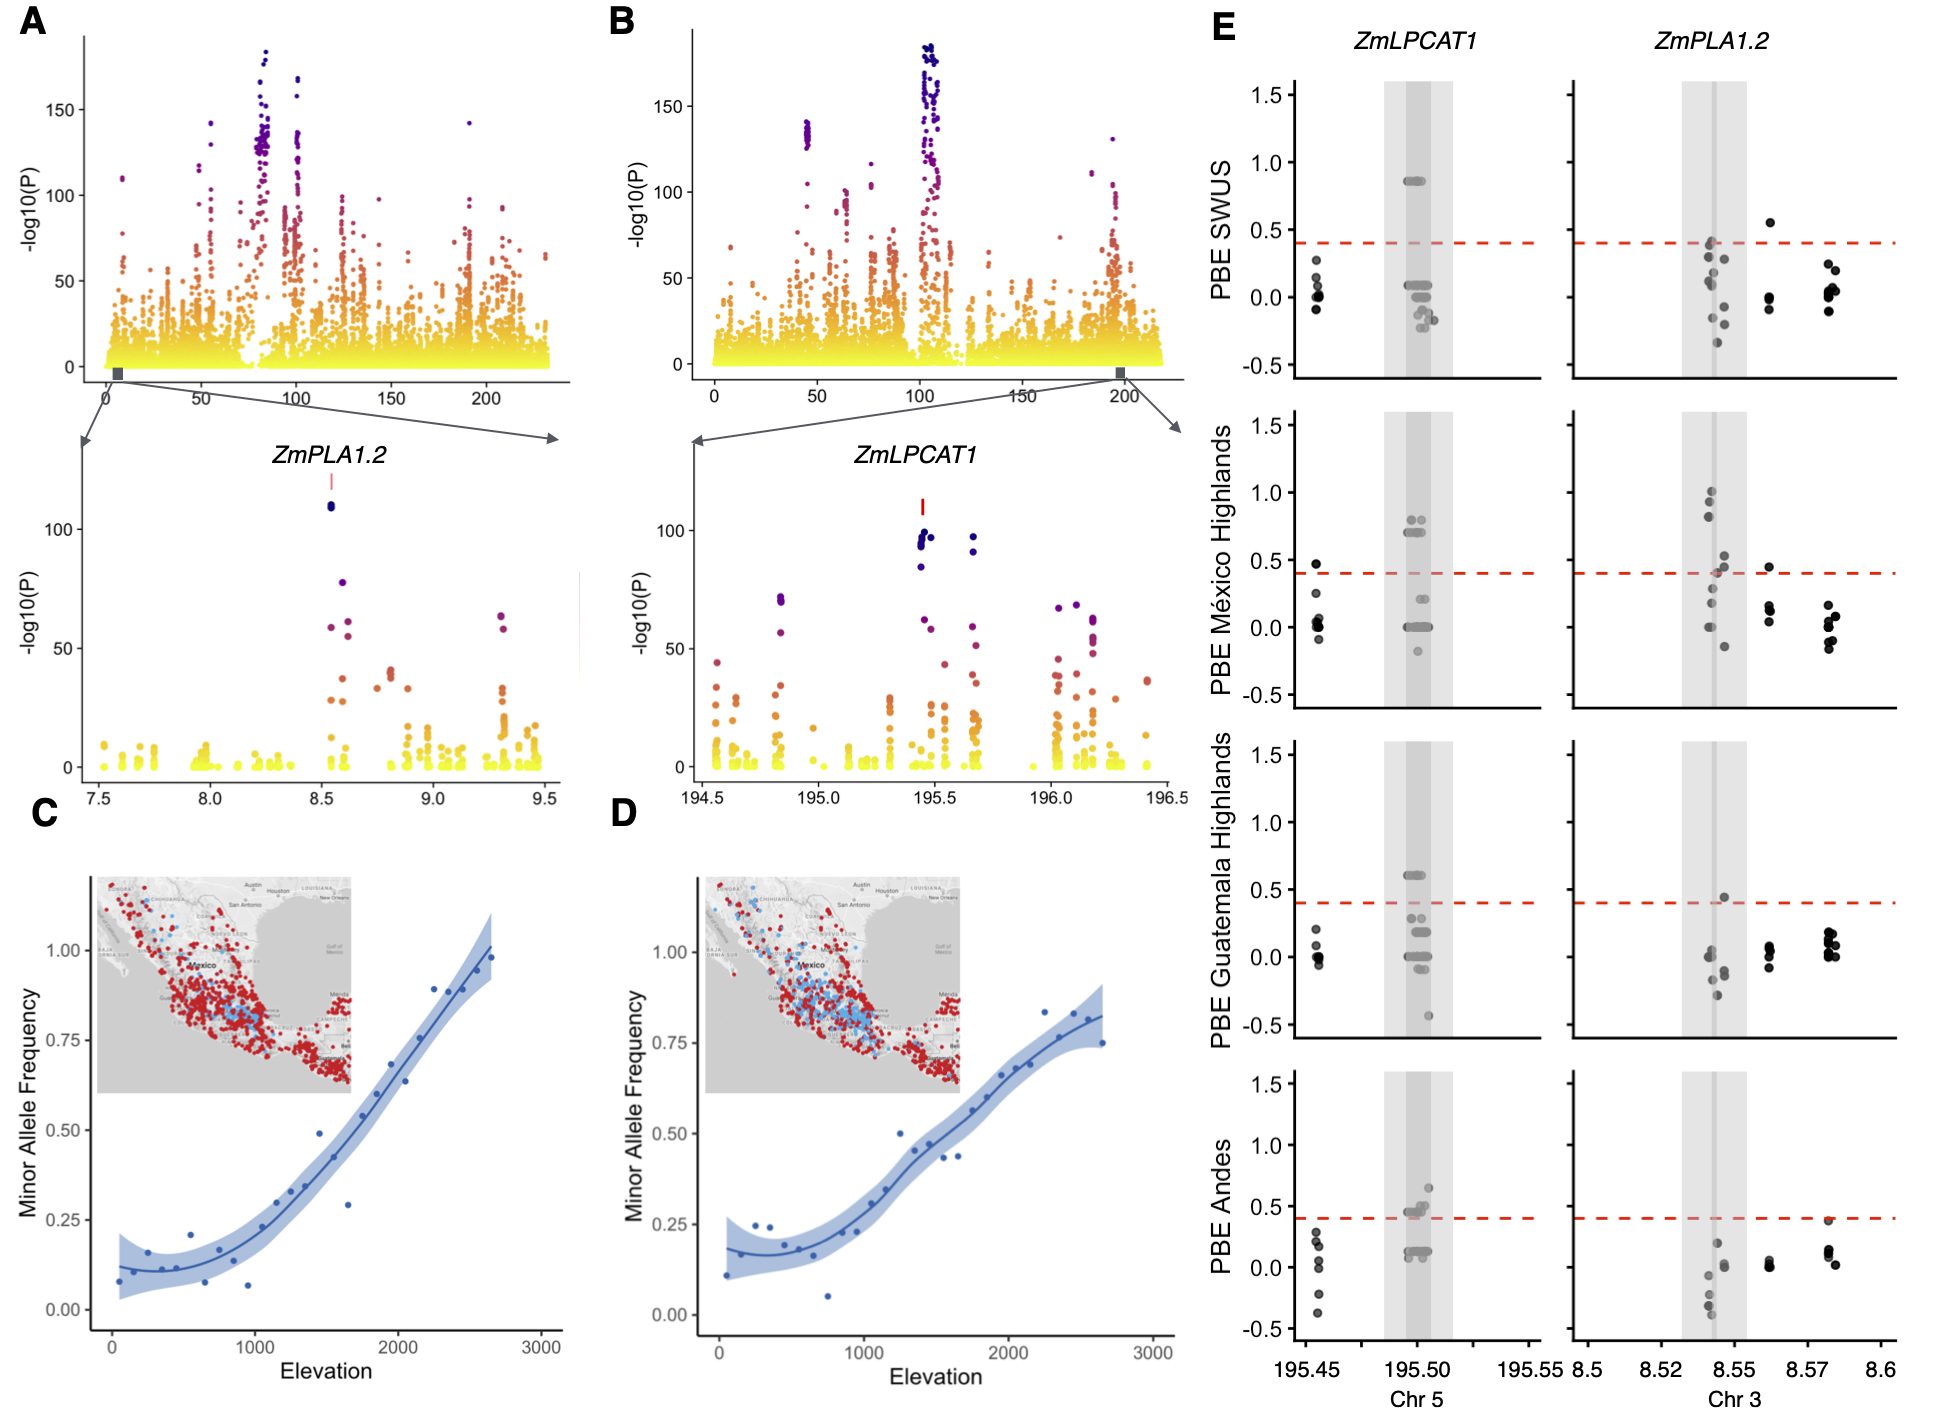
\includegraphics[width=0.4\paperwidth]{Figures/Fig_2.png}
\caption{Manhattan plots of minus log10(P‐values) \textit{Pcadapt} outliers. A) and B) \textit{Pcadapt} PC1 outliers plots of chromosome 3 and 5, respectively. 
Lower panels are zoomed areas of outlier SNPs that colocalize with the physical position of the coding sequences of \textit{ZmPLa1.2} and \textit{ZmLpcat1}. E) and F) show the geographic and elevation dependent frequencies of the highland (blue) and lowland (red) alleles of one of the outlier SNPs in the coding sequence of \textit{ZmPLa1.2} and \textit{ZmLpcat1}.}
\label{Fig2}
\end{center}
\end{figure} 

\subsection{QTL analysis of phospholipid content in a B73 x Palomero Toluqueño BIL mapping population identifies a major QTL explaining PC/LPC conversion} 

Our PBE and glycerolipid analysis of multiple highland and lowland populations across the Americas showed a strong signature of selection in genes involved in the synthesis and degradation of phospholipids. Glycerolipid analysis of the HiLo landrace diversity panel together with Qst-Fst results further supported that high PC/LPC ratios were selected for in highland maize from mesoamerica and to a lesser extend in South America.   
However, these results might be confounded by population structure that is commonly observed in maize landraces \cite{Romero_Navarro2017-cn}. 
To break population structure and further characterize selection and identify loci involved in glycerolipid synthesis in highland maize we developed a small (52 Backcross Inbred  Lines BC1S5), using B73 as the recurrent parent (75\% B73, 25\% PT). 
B73 is a temperate stiff-stalk inbred line. Palomero Toluqueño (PT) accession Mexi5 (CIMMYTMA 1567) is a popcorn (Palomero means popcorn in Spanish) highland landrace from the Toluca valley in México (Figure \ref{Fig3}G) 

The B73 x PT BC1S5 mapping population was grown in triplicate on the same common garden in Metepec, Edo de Mexico, Mexico as the 120 landrace diversity panel. The field site is only a few kilometers away from the original collection site of the Mexi5 accession. In this highland conditions, with typical 5 growth degree units across the growth season, Palomero Toluqueño shows higher fitness than B73 (Figure \ref{Fig3}E-G). While B73 typically flowers around 65 days after planting in US temperate conditions and Mexican lowland conditions B73 flowers around 150 days after planting in our Toluca field. 
Plants were sampled at the same time as the diversity panel for glycerolipid analysis. in the same way for glycerolipids analysis. 
Using the sum of lyso-phosphatydilcholines species (LPCs) we found a major QTL peak located at 8.5 Mb of chromosome 3 -qLPCs3- (Figure \ref{Fig3}A). 
We also found a major QTL peak -qLPCs3- when we use the sum of phosphatidylcholine species (PCs) (Figure \ref{Fig3}B). 
Effect size plots in this QTL peak show opposite genotypic behaviours. 
In the case of LPCs (Figure \ref{Fig3}B), BILS (Backcross Introgressed Lines) that are homozygous B73 at the QTL peak, have higher concentrations of LPCs that BILS that are homozygous PT. In the case of PCs (Figure \ref{Fig3}B), homozygous B73 BILS at the QTL peak have lower concentrations of PCs than homozygous PT BILS. 
The PCs/LPCs ratio also had a major QTL on the same region as qLPCs3 and qPCs3 with an even larger LOD. 

We then analyzed the correlation of the PCs/LPCs ratio and LPCs levels on the BILs and parental lines and found that PT shows high PC/LPC levels (Figure \ref{Fig3}C) like other Mexican highland landraces (Figure \ref{Fig1}E). 
As shown in the effect sizes plots in  Figure \ref{Fig3}B, BILs carrying the PT allele have low LPCs levels and high PCs levels. This data support the hypothesis the high PCS/LPCs ratios are characteristic of Mexican Highland landraces and that this is not driven by population structure. 

\begin{figure*}[!ht]
\begin{center}
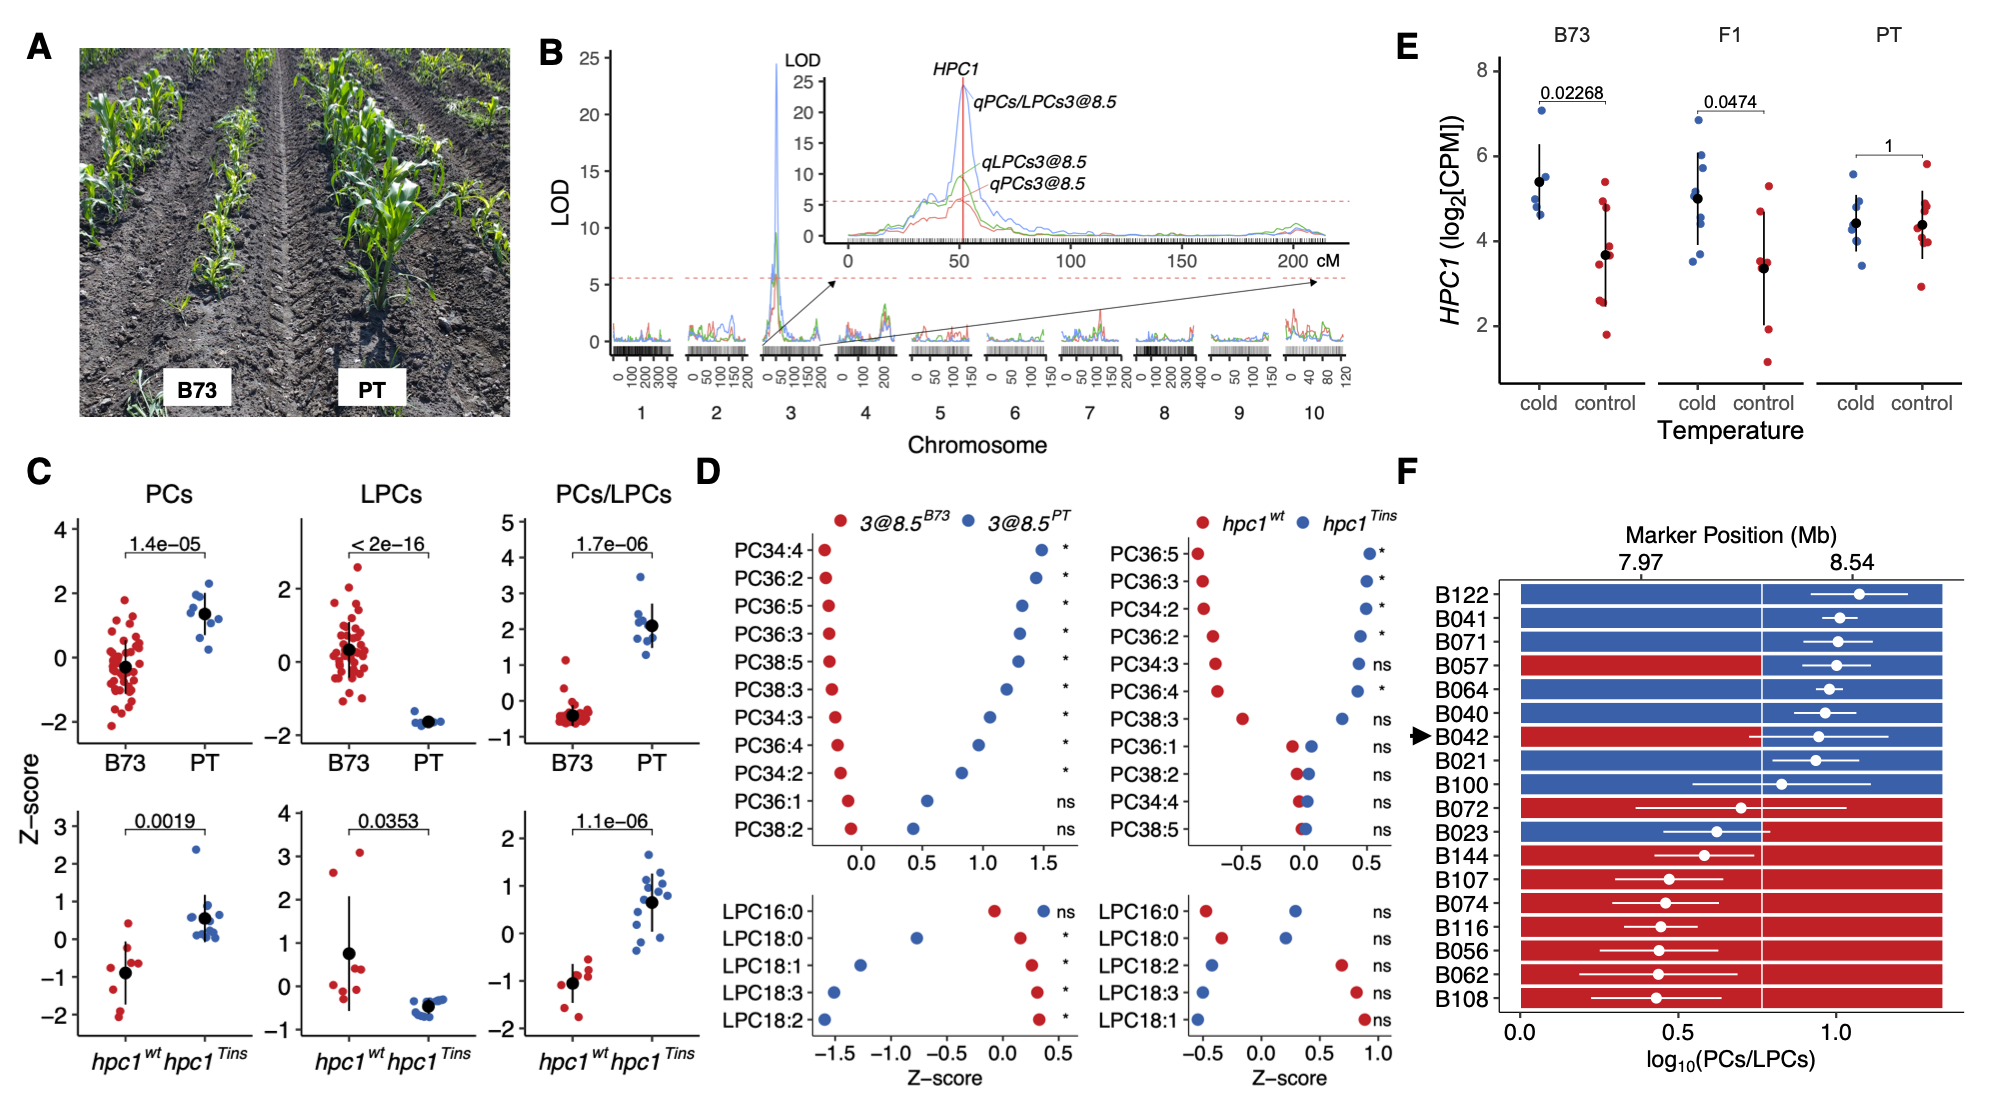
\includegraphics[width=0.8\paperwidth]{Figures/Fig_3.png}
\caption{Glycerolipid pathway selection 
A) Populations used in the Population Branch Excess (PBE)analysis. 
B) Average PBE values within genes and 10KB windows upstream and downstream of the gene of each pathway were compared against random genome wide sample of the same number of genes. The heatmap shows p-values of a (indicate what type of test) for each pathways. 
C) PBE values of SNPs in\textit{ZmLpcat1}and\textit{ ZmPla1.2}across SWUS, Mexican Highlands, Guatemalan Highlands an Andes populations (from top to bottom). Dark shade rectangles mark the coding sequence of each gene. Light shading rectanles on the borders of the coding sequence mark 10KB upstream and downstream windows. 
D) Map showing the geographical origin of the 120 accessions used in the common garden experiment to quantify glycerolipid compounds.
E) Correlation between  lyso-phosphatydilcholine (LPC) species and the ratio of  phosphatydilcholine (PCs) species and LPC species. 
F) Logaritmic values of the PC34:1/LPC18:1 ratio of highland and lowland landraces from Mesoamerica and Southamerica}
\label{Fig3}
\end{center}
\end{figure*} 
LPCs are the product of hydrolization of fatty acids from PCs by the action of A1 and A2 type phospholipases. A1 phospholipases hydrolize fatty acids on the SN1 position while A2 phospholipases hydrolize fatty acids on the SN2 position. 
PLC and D hydrolize the phosphocholine or choline polar groups of phosphatidylcholine.  
Based on these results we hypothesized that a gene coding for an enzyme controlling the PCs/LPCs ratio should be behind  qLPCs3 and qPCs3. 
We then used the B73 v3 genome assembly and identified 72 genes in the 7.9-10 Mb 99\% confidence interval around the QTL peak (Supp file 2). 
Among this list of genes, \textit{ZmPla1.2}, a gene with putative PLA1 function located right at the QTL peak (Chr3:8,542,107..8,544,078) is the most likely candidate underlying this QTL. 
There are 75 genes in the maize genome with predicted phospholipase activity and half of them have predicted PLA1 activity (Figure \ref{SupFig3}A). 
Using data from the B73 expression atlas \cite{Stelpflug2016-vr} we analyzed expression levels of all phopsholipases across 80 tissues in several developmental stages and found that \textit{ZmPla1.2} is one of the two most highly expressed phospholipases and is particularly highly expressed in the vegetative leaves between V4-V9. These are the same tissues we collected for glycerolipid analysis in our samples. 

\textit{ZmPla1.2} expression is highly upregulated in temperate inbred lines in seedlings exposed to cold stress and downregulated in heat stress (Figure \ref{SupFig3}C). 
Our PBE and \textit{pcadapt} identified \textit{ZmPla1.2} as gene under strong selection in highland maize. 
Our results of glycerolipid lipids in the landrace diversity panel also  indicated that the PCs/LPCs levels were particularly high Mexican highland landraces. 
We further studied PC, LPC selection using the individual species and individual PC/LPC species ratio. 
We found that most of the individual LPCs at the qLPCs3 locus correspond to LPCs that at contain at least one double bond in the fatty acid \ref{Fig3}D. The ratio of PC to LPC is higher in RILs that are homozygous PT at the \textit{ZmPla1.2} locus. The differences are most stark in ratios where the LPC lipid species is presumably a product of the reaction, as the reaction is not occuring in PT lines. For example, \textit{ZmPla1.2} would remove a 16:0 fatty acid from PC34:1 and leave LPC18:1 behind. We then used the Orr test of selection and found that PT allele significantly contributes to the high PC levels and low LPC levels. 

All taken together our PBE, pcapadapt, Qst-Fst and QTL data strongly suggest the PC-LPC balance was under selection and that \textit{ZmPLA1.2} and to a minor extent\textit{ZmLpcat1}are themselves under selection in highland maize and are major drivers of the lipid changes observed in highland maize. 
Furthermore, the QTL data suggest that the highland PT allele is a loss of function of \textit{ZmPLA1.2} as the levels of PCs are high in RILs in that region that are homozygous PT and LPC levels are low. 
This loss of function could be due to a mis-regulation of the expression level in highland landraces or to a mutation affecting the enzymatic activity of ZmPLA1.2. 
We analyzed \textit{ZmPLA1.2} expression in B73, PT and the F1 in plants grown under high and low temperature simulating highland and lowland conditions \cite{Crow2020-gene}. 
Under cold conditions \textit{ZmPLA1.2-B73} was upregulated (Figure 3\ref{Fig3}G). 
On the other hand \textit{ZmPLA1.2-PT} espression in cold conditions showed reduced variability when compared to warm conditions but was not significantly upregulated when compared with \textit{ZmPLA1.2-PT} in control conditions.
\textit{ZmPLA1.2-PT} expression in cold conditions was similar to \textit{ZmPLA1.2-B73} in control conditions.
\textit{ZmPLA1.2} on the F1 showed a pattern of expression consistent with a dominant B73 effect and this was also the case when we analyzed PC/LPCs ratios in the few B73 x PT BC1S5 BILs that are heterozygous at the qPC/LPC@8.5 locus. 
Loss of function could also be the result of enzymatic malfunction of the \textit{ZmPLA1.2-PT} allele and in fact PBE and pcadapt outliers SNPs are located within the CDS of \textit{ZmPLA1.2}. 
We Sanger sequenced B73 x PT BILs that are homozygous PT on the \textit{ZmPLA1.2} and we identified several SNPs that were already identify by GBS sequencing on the Seeds dataset and others that could have an effect on ZmPLA1.2. Non-synonimous SNPs are located 407, 520, 553, 610, 631, 1028, 1315, 1342, and 1345 basepairs into the CDS.
For example, SNP 631 is on the flap lid domain leading to a conservative substitution from isoleucine to valine. This could have an effect on the enzyme's activity since the flap lid domain controls substrate accessibility to the catalytic center. 

\subsection{\textit{ZmPla1.2} was introgressed in highland maize from \textit{mexicana} and this introgression is conserved northern US maize and northern European Flints}
The PT allele on the flap lid domain is highly conserved on Mexican and Guatemalan highland landraces used in the PBE analysis and segregates in the SWUS landraces. 
This is a typical pattern of teosinte \textit{mexicana} introgression \cite{Wang2020-mp} and indeed the PT allele was present in both teosinte \textit{mexicana} accessions sequenced in the maize hapmap. Interestingly, the PT allele was present in 1/4 of the teosinte \textit{parviglumis accessions on hapmap}. 
This lead us to ask whether the PT allele was the result of teosinte \textit{mexicana} introgression in highland maize or selected from \textit{parviglumis} standing variation in teosinte. To do this we used \(f_d\) data from \cite{Gonzalez-Segovia2019-jy} calculated using WGS of: two PT outbred individuals, a Mushito (another highland landraces) outbred individual, two lowland landrace inbreds, Reventador and NalTel, two \textit{mexicana} inbreds, three \textit{parviglumis} inbreds and a tripsacum individual used as an outgroup. 
\(f_d\) data around the \textit{ZmPla1.2} indicates that the region was introgressed from \textit{mexicana} into highland maize. (Figure\ref{Fig4}A).
\begin{figure}[!ht]
\begin{center}
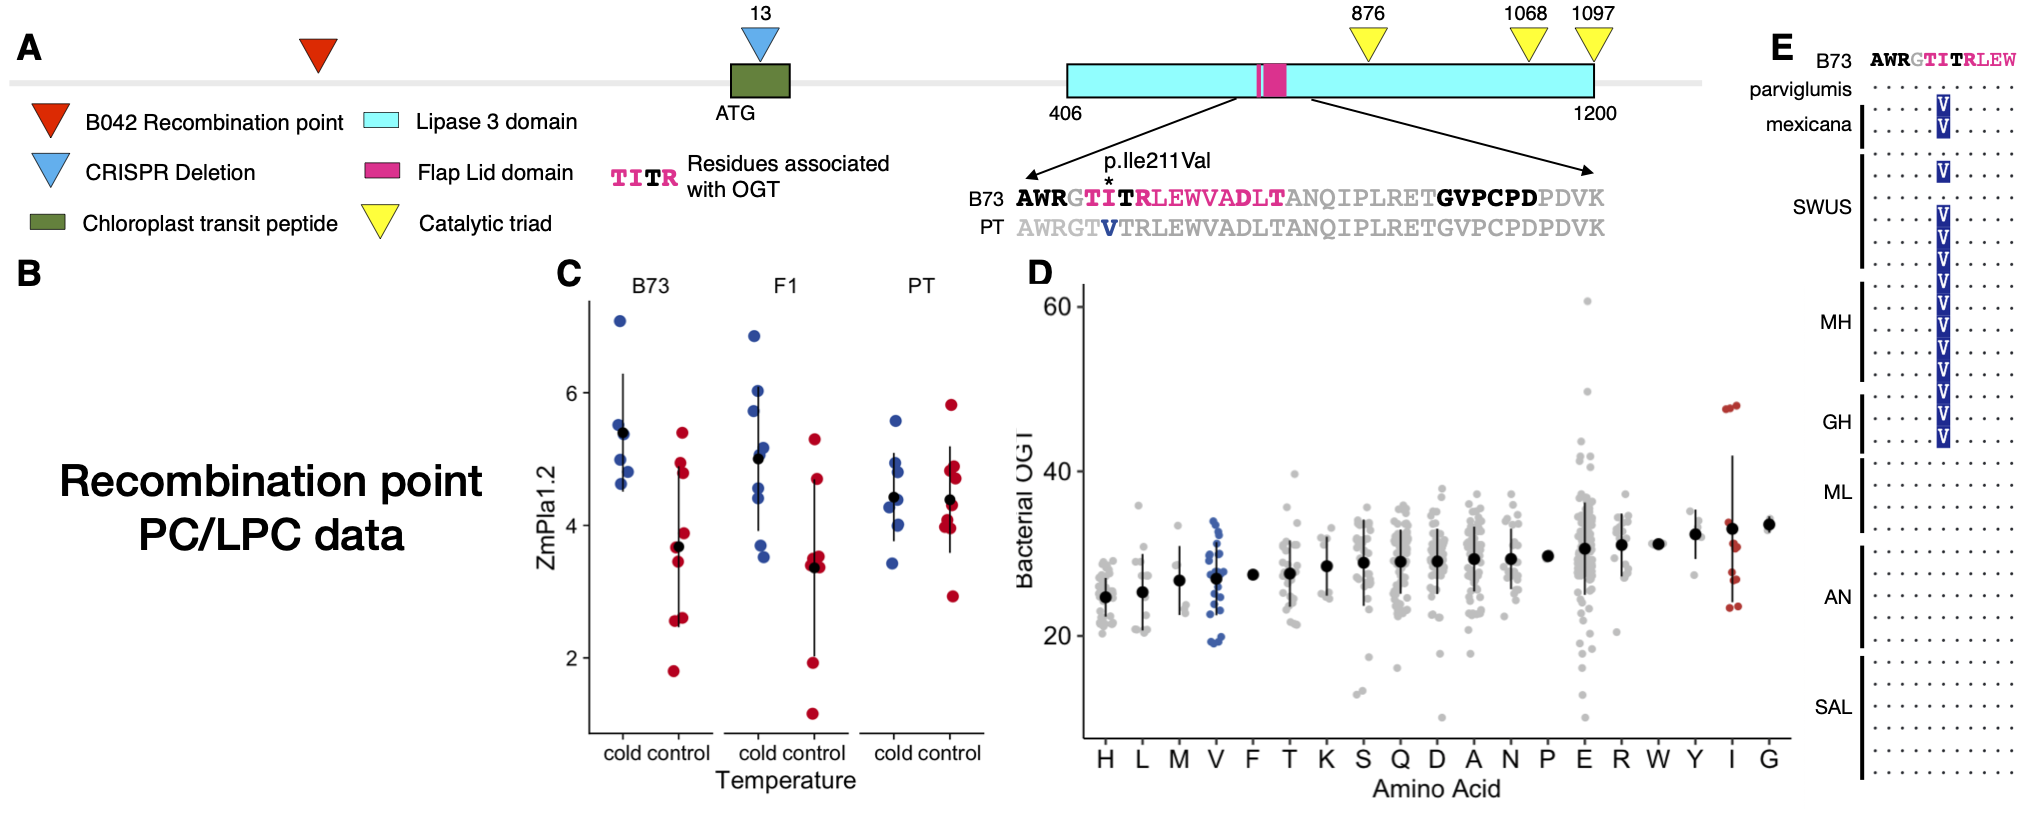
\includegraphics[width=0.43\paperwidth]{Figures/Fig_4.png}
\caption{Glycerolipid pathway selection 
A) \(f_d\) analysis of \textit{mexicana} introgression. Data was obtained from \cite{Gonzalez-Segovia2019-jy}. 
B) Haplotype network analysis of \textit{ZmPla1.2} CDS SNPs using X Mexican homozyogous individuals from the Seeds dataset.
C) Phyologenetic tree of \textit{ZmPla1.2} CDS using a sample of hapmap inbreds and Palomero Toluqueño} 
\label{Fig4}
\end{center}
\end{figure} 

We then performed a haplotype network analysis using SNP data of the \textit{ZmPla1.2} CDS from X Mexican homozygous accessions from the Seed Dataset \cite{Romero_Navarro2017-cn}. We identified 9 haplotype groups in an elevational gradient. The two major groups (II) and (VI) contained mainly lowland and highland landraces respectively. The two mexicana individuals were located in group IV together with a group of 7 highland landraces from X. 

We then asked if the mexicana introgression present in mesoamerican highland maize is present in modern inbreds. To adress this question we constructed phylogenetic tree using using sample of the hapmap inbred lines including lines from the 282 inbred panel and PT. Palomero Toluqueño and the teosinte \textit{mexicanas} TIL-08 and TIL-25 clustered together with Northern European Flints like EP1 UH008 and UH009. Other northern US flints like CM7 are also closely related to the mexican introgression. This data suggests that after introgression into highland maize, the mexicana introgression was conserved in Flint materials adapted to cold environments in the North of the US and Canada and Europe. 

\section{Materials and Methods}
\label{sec:materials:methods}

\subsection{Populations used in the analysis } 
Highland and lowland populations used for Population Branch Excess analysis consisted in three to six accessions from each of the populations and have been previously described in \cite{Wang2020-mp, Wang2017-bc}. 


The 120 Landraces from the HiLo Diversity Panel were selected and ordered from the \href{http://mgb.cimmyt.org/gringlobal/search.aspx}{CIMMYT germplasm bank} to maximize a good latitudinal gradient sampling across mesoamerica and South America. For each highland landrace (>2000 masl) a lowland (<1000 masl) was selected at the same latitude (<0.5$^{\circ}$) to form 60 highland/lowland pairs, 30 in each subcontinent. A list of the accessions used is provided in supplementary file  


B73 x PT BILs
Hilo Panel
Li genomes (can cite Li 2017)

We used landraces individual accessions genotypic data from the CIMMYT Seeds of Discovery project (SeeD). The SeeD project has genotyped 24,000 landraces from the  CIMMYT International Germplasm Bank maize collection primarily from American origin.


\subsection{Field Experimental Conditions and sampling} 
Two replicas of the Hilo Diversity panel accessions and three replicas B73 x PT BILs were planted in a field located in Metepec, Edo de Mexico, (19°13'28.7"N 99°32'51.6"W) within the Trans-Mexican volcanic belt. 
The field is at 2610 meters above sea level (masl), the range of average monthly temperatures along the year vary from 5 °C to 21.5 °C with an average annual of 13.6 °C.  
Fifty mg of fresh tissue was collected using a leaf puncher from the tip of the S2 leaf (two leaves younger of the last leaf with a fully developed collar), when the plants were around the V5 developmental stage. 
Tissue discs were immediately fast froze it in liquid nitrogen. All samples were collected in a single day between 10:00 am and 12:00 pm, approximately 3 h after sunrise. 
Samples were transported in dry ice to the lab and stored in -80 C until extraction. 

\subsection{Glycerolipid extraction and UHPLC-QTOF MS/MS lipid profiling} 
We collected fifty mg of leaf tissue  Frozen material was homogenized in a tissue grinder Retsch (Haan, Germany) for 40 seconds at a frequency of 30 1/s. After grinding, samples were extracted. 
We performed lipid extraction as reported by Matyash and collaborators (Matyash et al. 2008). 
First, 225 $\mu$L of cold methanol (MeOH), was added to each sample. 
For the blanks, MeOH previously prepared with a Quality Control (QC) mix was added (Supplementary Table XX). Each sample was vortexed for 10 seconds, keeping the rest of materials on ice. 
Then 750 $\mu$L of cold methyl tert-butyl ether (MTBE) were added. The MTBE added to the blanks contained 22:1 cholesterol ester as internal standard (Supplementary Table XX). 
Each sample was vortexed for 10 seconds, followed by 6 minutes of shaking at 4°C in the orbital mixer. 
188 $\mu$L of LC/MS grade water at room temperature (RT) was added, and the samples were vortexed for 20 seconds.
We centrifuged the samples for 2 min at 14000 rcf (12300 rpm) and recovered 700 $\mu$L of supernatant from the upper organic phase. 
We then split the supernatant two aliquots of 350 $\mu$L, one for lipid profiling and the other for preparation of pools to be used along the lipid profiling. 
Finally, samples were dried with a speed vacuum concentration system.
Dry samples were resuspended in 110 $\mu$L of MeOH-Toluene 90:10 (with the internal standard CUDA, 50 ng/mL). 
Samples were vortexed at low speed for 20 s and then sonicated at RT for 5 min. 
Aliquots of 50 $\mu$L per sample were transferred into an insert within an amber glass vial.
The UHPLC-QTOF MS/MS utilized were Agilent 1290 and Agilent 6530, respectively. 
Before analyzing the samples a new Waters Acquity charged surface hybrid (CSH) C18 2.1x100 mm 1.7 $\mu$m column was set. 
The column was initially purged for 5 min. 
The UHPLC column was coupled to a VanGuard pre-column (Waters Acquity CSH C18 1.7$\mu$m). 
Six “no sample injections” were injected at the beginning of each run to condition the column, followed by ten samples, one pool (made out of the mix of the second aliquot of all the samples contained per UHPLC plate) and one blank.
We injected 1.67 $\mu$L per sample into UHPLC-QTOF MS/MS ESI (+), the running time per sample was 15 min. Mobile phase “A” consisted of 60:40 acetonitrile:water, 10 mM of ammonium formate and 0.1\% formic acid. 
Mobile phase “B” consisted of 90:10 isopropanol:acetonitrile, 10 mM ammonium formate and 0.1\% of formic acid. 
The flow rate was maintained at 0.6 mL/min and the column compartment was maintained at 65 °C. Initial conditions were 15\% B; the gradient uniformly increased until reaching 100\%. 
At 12.10 min the mobile phase composition returned to initial conditions.
The mass spectrometer (QTOF MS/MS) was operated in positive electrospray ionization mode (ESI), based on the diversity and amount of lipid species identified under ESI (+) and (-) during the lipid profiling optimization (See supplementary Table 3) on Agilent® ultra high performance liquid chromatography and quadrupole time of flight mass spectrometry (UHPLC-QTOF MS). 
For this optimization we used 8 samples of B73, 8 samples of PT and 10 samples of a recombinant inbred line population (RILs) generated by crossing B73 and PT, only MS1 data was acquired. 
The same samples were utilized for both ESI modes. 
Under positive mode 24 lipids were identified, having two cholesterol esters (CE), 3 diacylglycerols (DG), 2 lysophosphatidylcholines (LPC), 10 phosphatidylcholines (PC), 1 phosphoethanolamine (PE) and 6 triacylglycerols (TG). 
While under negative mode we identified 16 lipids, of which, 14 were fatty acids (FA) and 2 were PC species. 
For the source parameters, ESI gas temperature was set at 325 °C, nebulizer pressure of 35 psig, gas flow of 11L/min, capillary voltage at 3500 V, nozzle voltage at 1000V, MS TOF fragmentor and skimmer at 120 and 65 V, respectively.
Under the acquisition parameters a mass range between 60 and 1700 m/z was set. As for reference mass parameters, a detection window of 100 ppm and a minimum height of 1000 counts were set. 

\subsection{Glycerolipid data processing}

We performed a retention time (rt) correction of the acquired data using Agilent MassHunter Qualitative Analysis® B.06.00 version and Microsoft Excel. 
To extract ion chromatograms (EICs) of the internal standards within the run we used Agilent MassHunter Qualitative Analysis.
We identified the time of the highest intensity point of each EIC, which then was used as the current retention time of the experiment. 
In Microsoft Excel, using the method retention time for internal standards and the current rt, a polynomial regression was performed to obtain an equation that was used for calculating new retention times for 501 lipids listed in a MS1 m/z-rt library from Dr. Oliver Fiehn laboratory (See Supplementary Table 2). 
To identify other lipid species we decided to perform un-targeted MS/MS to explore in the lipid diversity within the samples. 
To acquire MS/MS data we selected 36 samples from the study to be run across four m/z ranges: 120-300, 300-600, 600-900 and 900-1200. 
From this MS/MS data, we used MSDIAL \cite{Tsugawa2015-kh} to check for false positives by analyzing how many fragments of each identified lipid matched the spectra from \textit{lipidblast} library (Kind et al. 2013). 
After this, we were able to add 339 new annotations into the mz-rt library, ending up with a total of 840 lipids species within this library which later were used to reprocess the spectra using MSDIAL and MS-FLO \cite{DeFelice}. 
Acquiring MS/MS data allowed us to identified additional lipid species, that we were not able to detect using only MS1 data, like monogalactosyldiacylglycerols (MGDG), digalactosyldiacylglycerols (DGDG) and plasmenylphosphatidylcholine (plasmenylPC). 
Within MSDIAL \cite{Tsugawa2015-kh}. Identification of lipids is based on two approaches: the MSP file and MS/MS identification setting included within the software and the use of a post identification file containing accurate m/z and rt for a list of lipids. In this study we used both identification approaches. 
The MSP file and MS/MS identification setting has a total of 51 lipid classes, under positive ion mode, that can be selected for identification. 
The post identification file that we used was the retention time-corrected MS1-MS2 mz-rt lipid library that we explained before. 
We used MSDIAL \cite{Tsugawa2015-kh} version 3.40. To use MSDIAL, the raw data was converted from .d to .abf format with Reifycs Abf converter (https://www.reifycs.com/AbfConverter/). The MSDIAL alignment results were filtered out based on whether compounds intensity was ten times above blank intensity. Then, filtered data was normalized using Systematic Error Removal using Random Forest (SERRF) \cite{Fan2019}, this normalization is based on the quality-control pool samples used along the study. Normalized features were filtered out considering a coefficient of variation (CV) equal or less than 30\% along the pools. To curate the data for duplicate features, isotopes and ion-adducts we utilized MS-FLO \cite{DeFelice}. Curated data was also normalized using sum known metabolite signal (mTIC), in Excel software.

\subsection{Population Branch Excess Analysis}

\subsection{\textit{Qst-Fst} analysis of glycerolipid data}

\subsection{\textit{pcadapt} analysis of biological adaptation in Mexican landraces}

\subsection{QTL analysis of glycerolipid levels}

\subsection{Orr test of selection of phospholipid levels}

\subsection{Teosinte \textit{Mexicana} introgression in highland maize}

\subsection{Haplotype network analysis of \textit{ZmPla1.2} in Mexican maize landraces and teosintes.}

\subsection{Phylogenetic analysis of\textit{ZmPla1.2} in maize inbreds and teosintes.}
Using v3 of B73 genome, SNPs occurring in PLA1.2 were obtained from SNPversity on MaizeGDB for the 282 genotype, German, and TIL datasets. SNPs were aligned using Geneious2020.0.5 and a neighbor-joining phylogenetic tree was generated. To make a more viewable tree, those with identical SNPs were condensed into one branch. The tree was further condensed by choosing only representatives from diverse geographic locations to display. Removed genotypes can be found in supplemental materials. 
\subsection{Association of \textit{ZmPla1.2} with agronomic traits}
We re-analyzed phenotypic data from the F1 Association Mapping (FOAM) panel of Romero-Navarro \textit{et al} \cite{Romero_Navarro2017-cn} and Gates \textit{et al} \cite{Gates2019-xu} to more fully characterize associations signatures of \textit{ZmPla1.2}. 
Full descriptions of this experiment and data access are described in those references. 
We downloaded BLUPs for each trait and line from Germinate 3, and subsetted to only those lines with GBS genotype data from Mexico. 
We fit a similar model to the GWAS model used by Gates \textit{et al} \cite{Gates2019-xu} to estimate the effect of \textit{ZmPla1.2} genotype on the trait's intercept and slope on trial elevation, accounting for effects of tester ID in each field and genetic background and family effects on the trait intercept and slope using four independent random effects. 
We implemented this model in the \textit{R} package \textit{GridLMM} \cite{GridLMM2019}. 
We extracted effect sizes and covariances conditional on the REML variance component estimates and used these to calculate standard errors for the total \textit{ZmPla1.2} effect as a function of elevation. 
To test whether the phenotypic effects of \textit{ZmPla1.2} on yield components could be explained as indirect effects via flowering time, we additionally re-fit each model using Days-To-Anthesis as a covariate with an independent effect in each trial.

\subsection{CRISPR-CAS9 editing of ZmPla1.2 and analysis of the effect of pla1.2 mutant on flowering time}

\subsection{Data Availability}

At the end of the Materials and Methods section, include a statement on reagent and data availability. Please read the Data and Reagent Policy before writing the statement. Make sure to list the accession numbers or DOIs of any data you have placed in public repositories. List the file names and descriptions of any data you will upload as supplemental information. The statement should also include any applicable IRB numbers. You may include specifications for how to properly acknowledge or cite the data.

For example: Strains are available upon request. File S1 contains detailed descriptions of all supplemental files. File S2 contains SNP ID numbers and locations. File S3 contains genotypes for each individual. Sequence data are available at GenBank and the accession numbers are listed in File S3. Gene expression data are available at GEO with the accession number: GDS1234. Code used to generate the simulated data is provided in file S4. 


\section{Discussion}
\label{sec:discusion}

\section{Acknowledgments}
\label{sec:acknowledgments}

\bibliography{bibliography}

\pagebreak

\section*{Supplemental Tables and Figures}

\renewcommand{\thefigure}{S\arabic{figure}}
\linenumbers

\setcounter{figure}{0}

\begin{figure*}[t]
\begin{center}
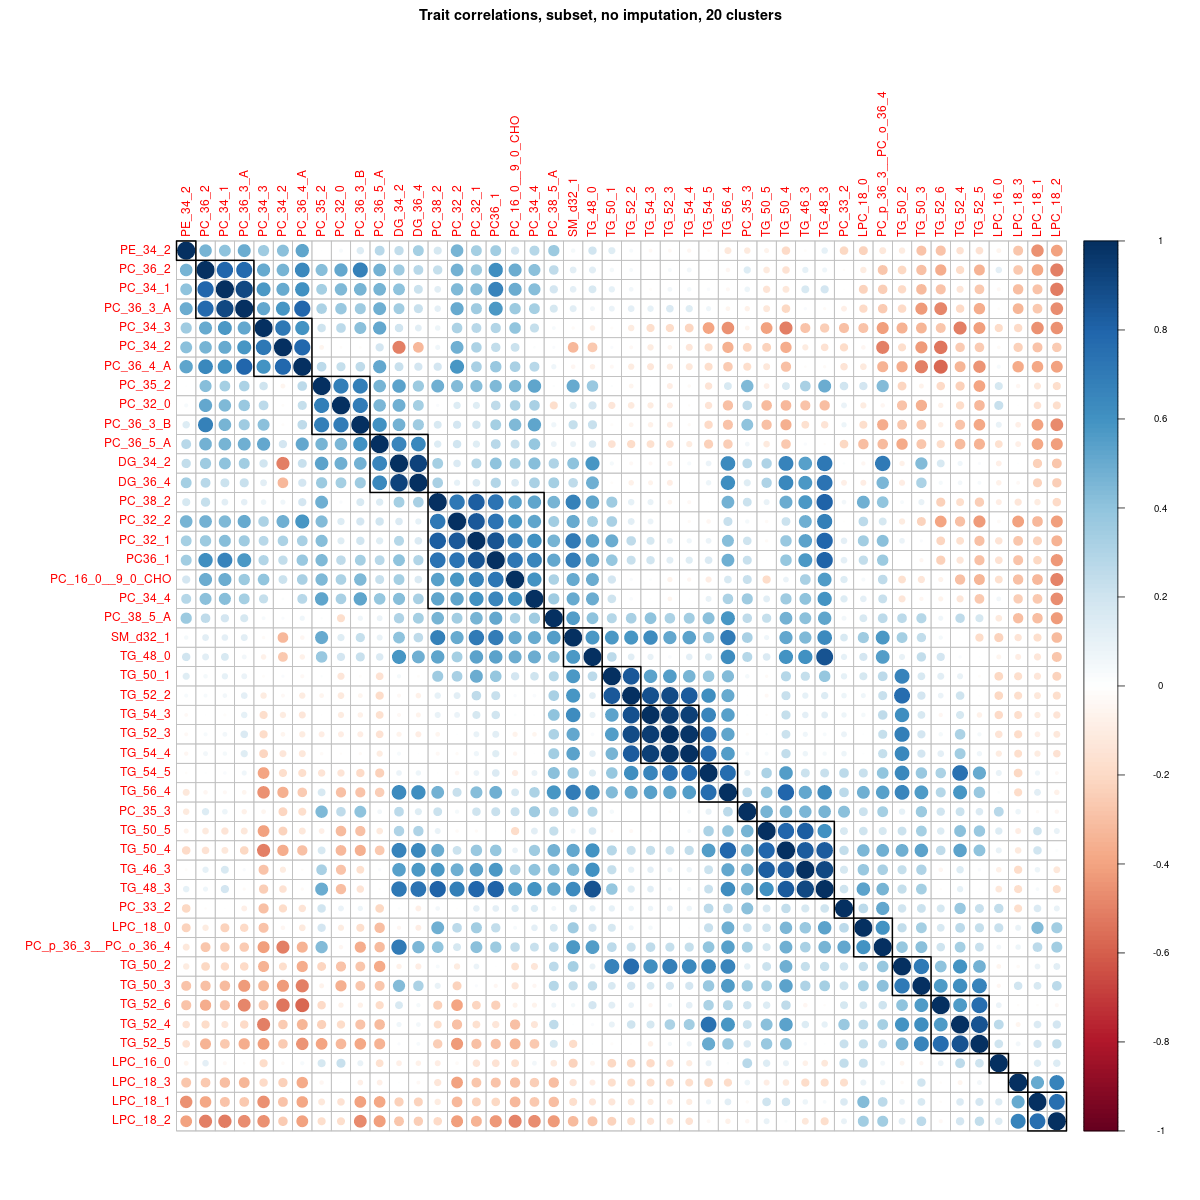
\includegraphics[width=0.8\paperwidth]{Sup_Figures/Sup_Fig_1.png}
\caption{A) Population Branch Excess Analysis of glycerolipid pathway genes. From the initial set of 211 genes we used 186 genes with 6219 non redundant SNPs and 683162 non redundant SNPs for the SW US group; 186 genes with 6106 non redundant SNPs and 664555 non redundant SNPs for the Mexican Highland group; 185 genes with 5912 non redundant SNPs and 641186 non redundant SNPs for the Guatemalan Highlands group; and 184 genes with 5698 non redundant SNPs and 614783 non redundant SNPs for the Andes group.    
\textit{Qst-Fst} analysis of glycerolipid compounds between highland and lowland landraces from Mesoamerica (B) and South America (C). Samples for Dart-Seq genotyping were taken from the same plants that were grown in the common garden experiment shown in Figure 1D-F and that were used for glycerolipid analysis   
}
\label{SupFig1}
\end{center}
\end{figure*} 

\begin{figure*}[t]
\begin{center}
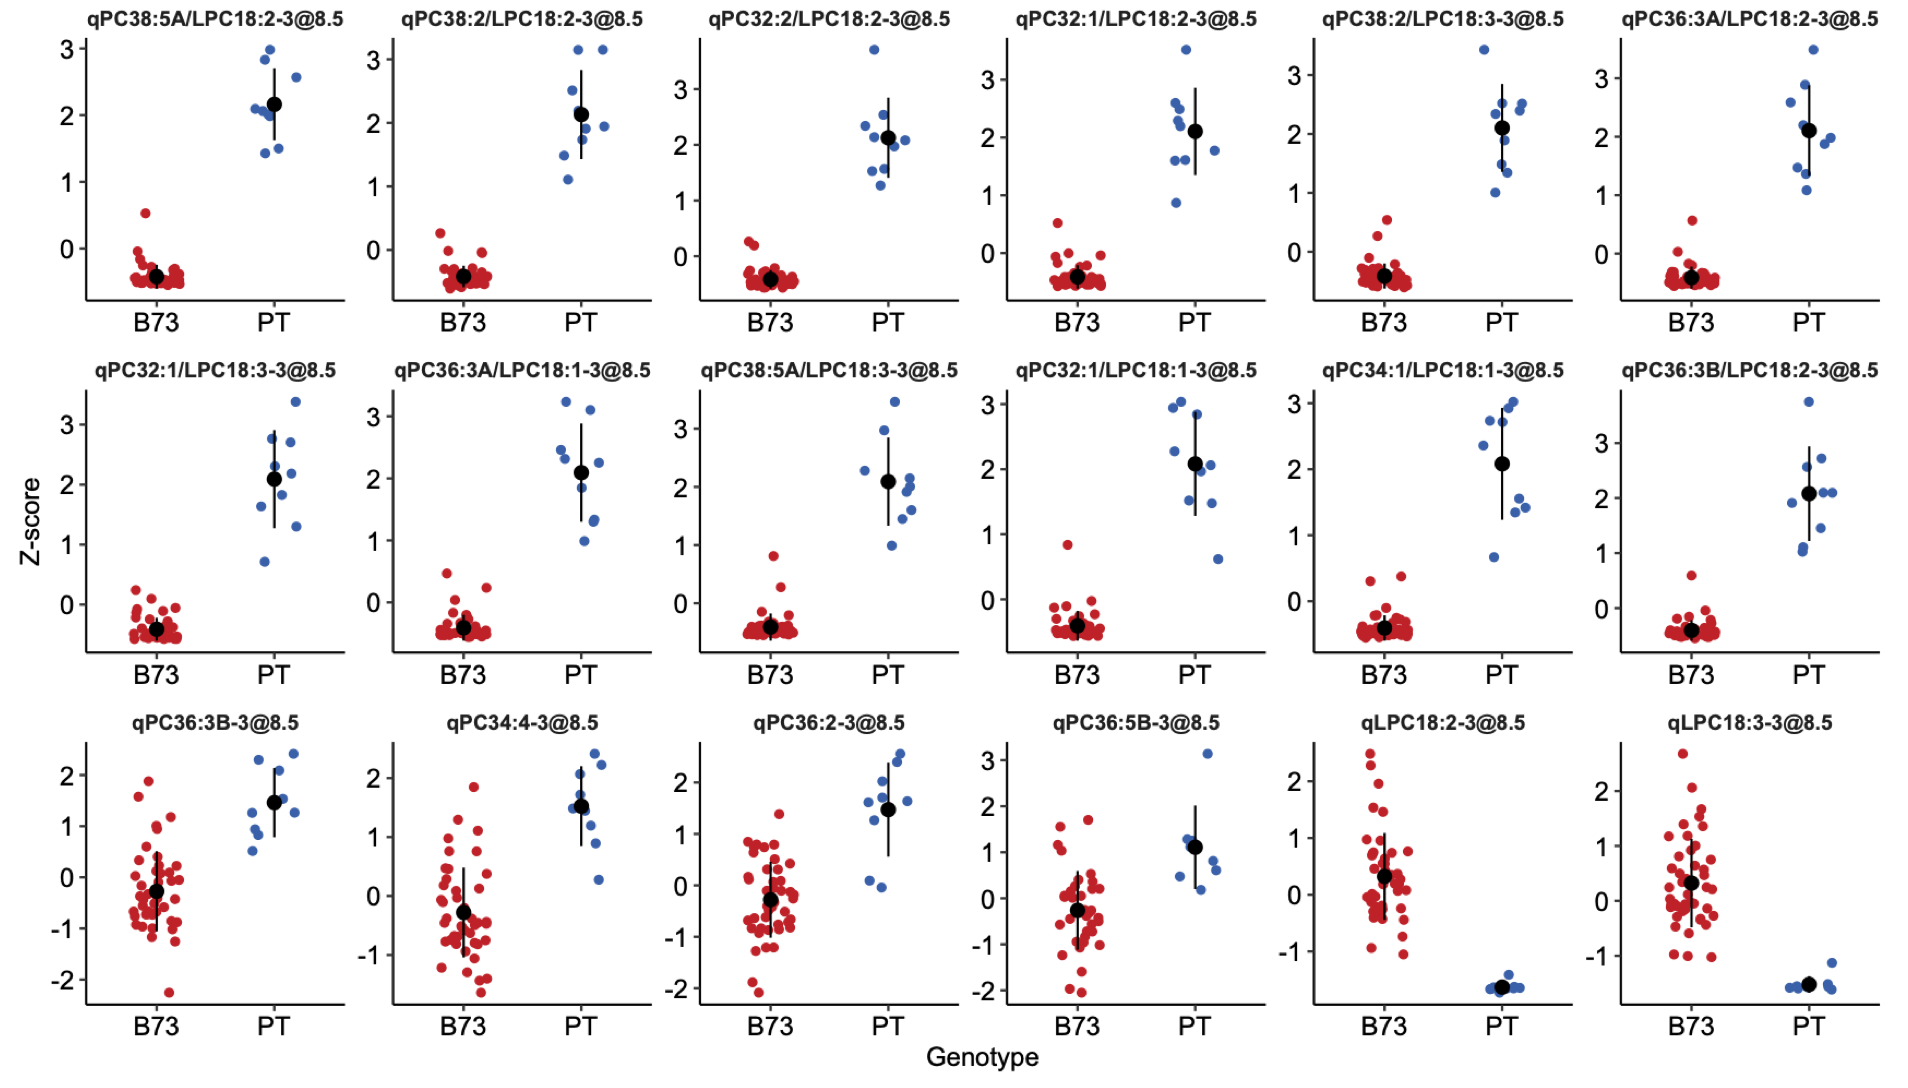
\includegraphics[width=0.8\paperwidth]{Sup_Figures/Sup_Fig_2.png}
\caption{\textit{Pcadapt} analysis of Latin America Landraces. We used GBS data from the Mexican landraces of the SEEDs dataset \citep{Romero_Navarro2017-cn} and run a \textit{pcadat} analysis \citep{Luu2017-ws} that identified (A) elevation as the major driver of population differentiation polarizing PC1.  
B) Genome wide analysis of \textit{Pcadapt} PC1 outliers. 
C) Distributions of pcadapt -log10(p values) of PC1 probabilities in a random sample with the average value of pcadapt scores from the glycerolipid PBE outlier genes of each of the four highland populations. 
}
\label{SupFig2}
\end{center}
\end{figure*} 

\begin{figure*}[t]
\begin{center}
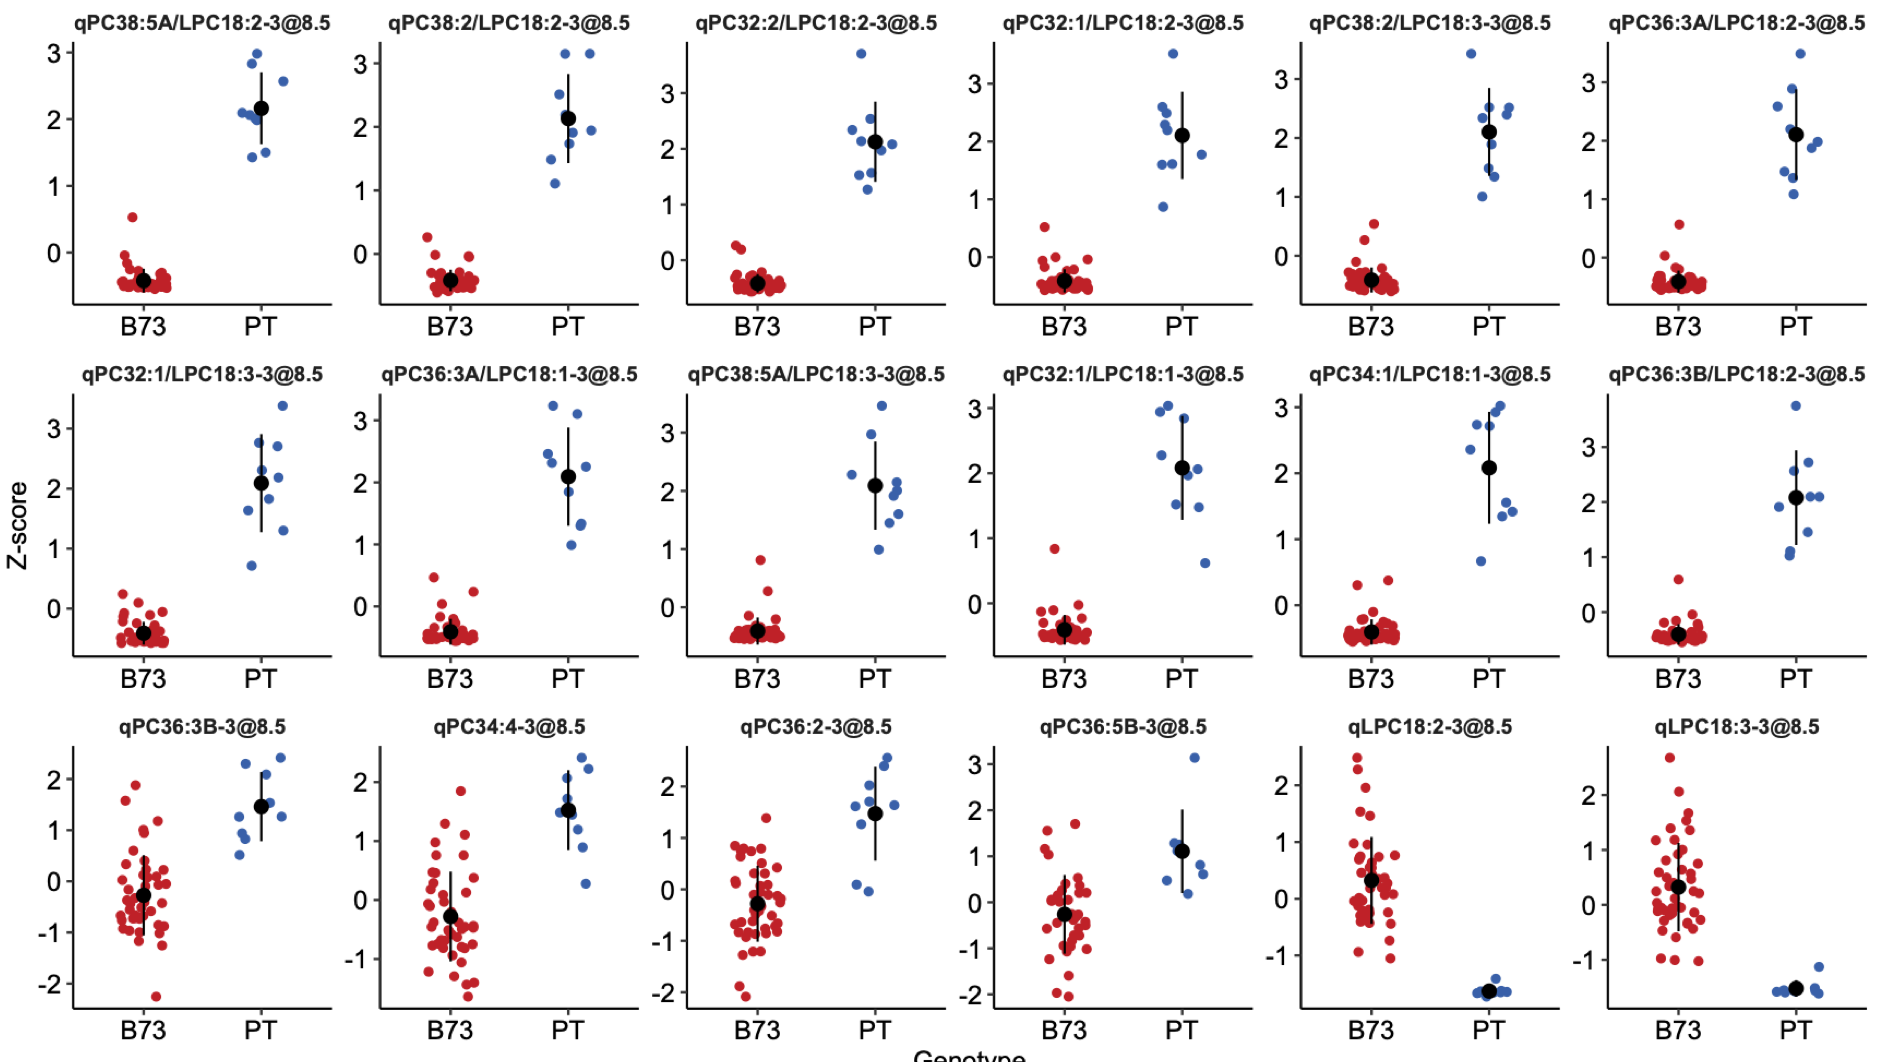
\includegraphics[width=0.8\paperwidth]{Sup_Figures/Sup_Fig_3.png}
\caption{A) Genomic Location of genes coding for enzymes predicted Phospholipase A1 activity. B) B73 expression levels of genes coding for enzymes with predicted Phospholipase A1 activity across different tissues. \textit{ZmPla1.2} is indicated in blue. C) \textit{ZmPla1.2} expression levels of temperate inbreds B73, Mo17, Oh43, and Ph207 under control, control and heat stress. Values taken from \cite{Waters2017-nat}. D) \textit{ZmPla1.2} and \textit{ZmLpcat1} expression levels correlations in the base of leave 3 in the 282 maize diversity pane \cite{Kremling2018-gn}. 
}
\label{SupFig3}
\end{center}
\end{figure*}  

\begin{figure*}[t]
\begin{center}
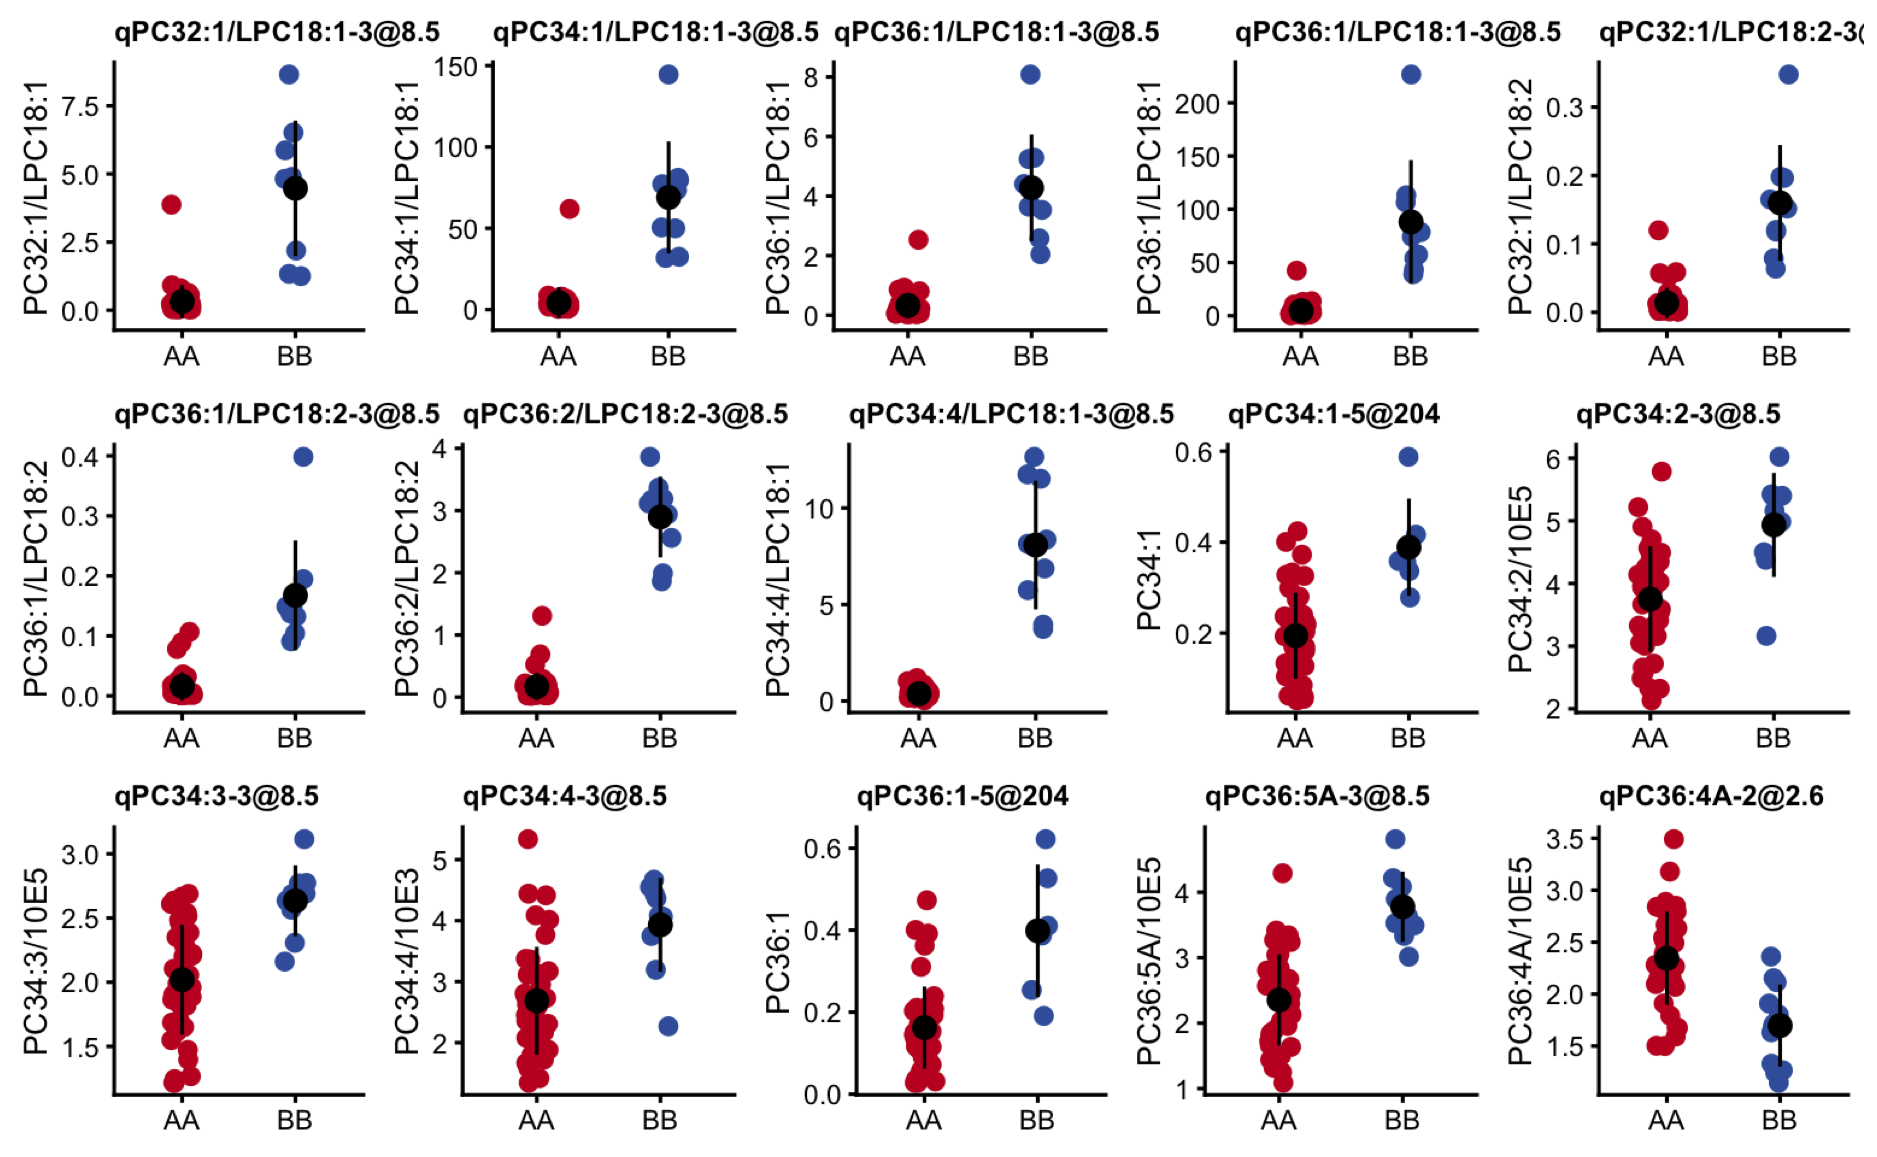
\includegraphics[width=0.8\paperwidth]{Sup_Figures/Sup_Fig_4.png}
\caption{A) \textit{ZmPla1.2-B73} sequence with Palomero Toluqueño synonimous and non-synonimous SNPs indicated in grey and orange respectively. The main domains including the lipase domain, the catalytic tria, the flap lid and the nucleophilic elbow are marked. B) Protein sequence alignment the flap lid domain and the catalytic triad in several species.  
}
\label{SupFig4}
\end{center}
\end{figure*}  




\end{document}